\documentclass[10pt,a4paper]{article}
\usepackage[utf8]{inputenc}
\usepackage{amsmath}
\usepackage{amsfonts}
\usepackage{amssymb}
\usepackage[]{algorithm2e}
\usepackage{graphicx}
\begin{document}

\title{LINGI2261: Artificial Intelligence \\
Assignement 1 : Solving Problems with Uninformed Search - Numberlink Project}
\author{Ndizera Eddy \and El Jilali Solaiman}
\date{\today}
\maketitle

\section*{Introduction}

\section{Python AIMA}

Here are the answers to the questions regarding the AIMA library.

\begin{enumerate}
	\item \textbf{In order to perform a search, what are the classes that you must define or extend ? Explain precisely why and where they are used inside a tree\_search.} \\

	
	In order to perform a search, the \textbf{Problem} class must be defined. We'll have to implement the following 3 methods  \textit{init}, \textit{goal\_test} and \textit{successor}. \\
	To explain why and where they are used inside a tree\_search, i'll use the pseudocode for a tree\_search (found in the textbook of the course "IA: A modern approach").\\
	
		
\begin{figure}[!h] %on ouvre l'environnement figure
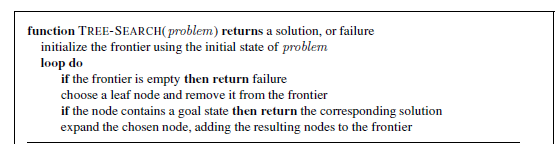
\includegraphics{Tree-Search.png} %ou image.png, .jpeg etc.
\caption{Tree-Search from \textit{Artificial Intelligence a Modern Approach}} %la légende
\label{image_soleil} %l'étiquette pour faire référence à cette image
\end{figure} %on ferme l'environnement figure 
	
	In the pseudocode, we see that to initialize we need the initial state of the problem. This initial state is given by the \textit{init} method found in the \textit{Problem} class.\\
	At line 5 of the same pseudocode, to know if we reach the goal, the \textit{goal\_test} method should be called to know that.\\
	Finally, the method \textit{successor} is called at the last line of the pseudocode to expand a node.\\
	
	This pseudocode looks like the method \textit{tree\_search} in the \textit{search.py} file.\\
	
	Also we need to implement the class \textbf{State} that represents the state of the problem given an action. The state is maintained in the node and it is important so that we keep track of the evolution of the problem. Also it facilitate us to know if we reach the goal state. \\
	
	
	\item \textbf{In the expand method of the class Node what is the advantage of using a yield instead of building a list and returning it afterwards?} \\
	
	In python, the \textit{yield} operator allows us to perform \textbf{lazily}. Indeed the call to the lazy operator do only one thing: returning a generator object that will be call later. It allows us to give out new values on the fly and to save memory space.\\ 
	
	
	\item \textbf{Both breadth\_first\_graph\_search and depth\_first\_graph\_search are matking a call to the same function. How is their fundamental difference implemented?} \\
	
	The fundamental difference between the two functions is the type of queue that they put as parameter when calling the function \textit{graph\_search}. The first one (breadth) put as queue a \textit{FIFOQueue} whereas the second one (depth) use a \textit{Stack} \textit{LIFOQueue}.\\
	
	With a \textit{LIFOQueue} the last most recently generated node is chosen for expansion. It implies that we explore first completely a branch before passing to another according to the definition of depth first tree search. \\
	
	With a \textit {FIFOQueue} the first generated node is chosen for expansion. It implies that  we explore first all the nodes of a specific depth according to the definition of breadth first tree search.\\
	
	\item \textbf{What is the difference between the implementation of the graph\_search and the tree\_search methods and how does it impact the search methods?}\\
	
	The difference between the tree\_search and the graph\_search is the variable \textit{closed} that is a data structure that records the nodes (states) already visited. It ensures us to avoid the infinite loop problem (occuring in depth\_first). 
	
	\item \textbf{What kind of structure is used to implement the closed list? What are the methods involved in the search of an element inside it? What properties must thus have the elements that you can put inside the closed list ?} \\
	
	The closed list is implemented using a \textbf{dictionnary}. It uses a pair (key, value) to store elements. The \textit{key} is used to search (like an index) the \textit{value}. \\
	
	To search an element, the hash value of the object used as key 
	
	The elements must be comparable?, unique?, immutable?.
	
	\item \textbf{How technically can you use the implementation of the closed list to deal with symmetrical states ? }\\
	
	By modifying the \textit{hash} and \textit{eq} method of the type used as key (a State object in our case) as so two symmetrical states give the same hash and are considered equals.
		
\end{enumerate}

\section{The Numberlink Problem}

\begin{enumerate}
	
	\item \textbf{ Explain the advantages and weaknesses of the following search strategies on this problem (not in general): depth first, breadth first.} \\
	
	The depth first search in general takes less time than the breadth first one. Also in this particular problem, the depth first has the completness property like the breadth first because there cannot have infinite search (if the grid is filled then the branch stops there). \\
	
	For the space occupied by the two search algorithm, this is not a issue because we use a yield to expand a node and not a list. \\
	
	The breadth first is advantageous with trees that have a high branching factor.
	%Me semble incomplet
	
	\item \textbf{How can we exploit the uniqueness of solution to reduce the search space? Why is the method pathExists useful?} \\
	
	The fact that the solution is unique reduces the search space because we can stop our search when  we found a solution that respects the condition given. We don't need to search a solution that could be more optimal because there isn't another solution. \\
	
	The method pathExists is useful to know if a a current node won't give a solution to the problem. Indeed, we can check , for example, for all paths if their two endpoints can be joined. If the check gives a negative response, then we can say that this node won't give a solution. It's a waste of time to expand this node.\\	
	
	\item \textbf{Is the order in which we choose the paths important? How can we use this to reduce the search space? When starting a new path, we can choose to start with any of its two endpoint. How should this choice be done?} \\
	
	Yes, it's important. Depending of the order, we can reduce the search space. Consider path A that has its two endpoints separated by a distance of 2 (number of points that separate them) and path B that has its two endpoints separated by a distance of 15. It would be wiser to begin constructing path A than path B .\\
	
	The choice of endpoints is also important because if we consider path A that has its two endpoints on the same line for example. If we expand the nodes by the following actions in that order : left, right, up and down. The faster solution is to pick the endpoints that is rightmost.\\
	
	\item \textbf{What are the advantages and disadvantages of using the tree and graph search for this problem. Which approach would you choose? Which approach allows you to avoid expending twice symmetrical states?} \\
	
	The tree search takes less time in case that the problem cannot have symmetrical states. But the graph search could save time in case symmetrical states are present in the search. \\
	
	The tree search doesn't lose time in checking if the current node has already been visited. Note that this problem cannot have infinite loop (explain why). \\
	
	We will choose the graph search approach. 
	
	\item \textbf{Implement this problem in Python 3. Extend the Problem class and implement the necessary methods and other class(es) if necessary. Your file must be named numberlink.py. You program must take as only input the path to the init file of the problem to solve. It must print to the standard output a solution to the problem satisfying the above format. Your file must be encoded in utf-8. Submit your program on INGInious.} \\
	
	\item \textbf{Experiments must be realized with the 10 instances of the numberlink problem provided. Report in a table the results on the 10 instances for depth-first and breadth- first strategies on both tree and graph search (4 settings). You must report the time, the number of explored nodes and the number of steps from root to solution. When no solution can be found by a strategy in a reasonable time (3 min), explain the reason (time-out and/or swap of the memory). What do you conclude from those experiments?} \\
	

\end{enumerate}

\section*{Conclusion}

\end{document}